% 2010 年福建卷文科第 15 题：四个平面点集（阴影区域及其边界），判断其中哪些为凸集。
% 来源 PDF：普通高考/2010/2010福建文.pdf，SHA-256 56e9e7a7fe9733a605b2d88773e59f83f49c173184cc77d721633adf13c16b78。
% 原页：第 1 页（A3 三栏）第 2 栏下部，书页码 591。
% 重绘依据：照原页四图自左至右排列——① 带凹顶点的多边形（箭头形，非凸）；
%   ② 一条线段；③ 由一段圆弧与其弦围成的弓形（小于半圆，凸）；
%   ④ 两个外切圆（两圆的并，非凸）。阴影为灰色，四图下方依次标注序号 ①—④。
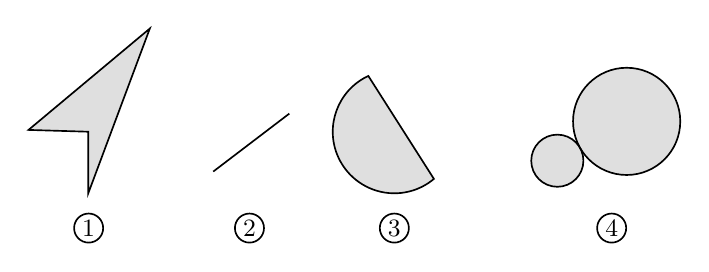
\begin{tikzpicture}[scale=0.92, semithick]
  % ① 凹多边形（有一处凹顶点）
  \fill[gray!25] (0,0.875) -- (1.675,2.275) -- (0.825,0) -- (0.825,0.85) -- cycle;
  \draw (0,0.875) -- (1.675,2.275) -- (0.825,0) -- (0.825,0.85) -- cycle;
  % ② 线段
  \draw (2.55,0.30) -- (3.60,1.10);
  % ③ 弓形：圆弧与其弦
  \fill[gray!25] (5.05,0.85) ++(115:0.85)
    arc[start angle=115, end angle=310, radius=0.85] -- cycle;
  \draw (5.05,0.85) ++(115:0.85)
    arc[start angle=115, end angle=310, radius=0.85] -- cycle;
  % ④ 两个外切圆
  \fill[gray!25] (7.30,0.45) circle (0.36);
  \fill[gray!25] (8.257,0.993) circle (0.74);
  \draw (7.30,0.45) circle (0.36);
  \draw (8.257,0.993) circle (0.74);
  % 序号
  \node[circle,draw,inner sep=1.1pt,font=\small] at (0.83,-0.48) {1};
  \node[circle,draw,inner sep=1.1pt,font=\small] at (3.05,-0.48) {2};
  \node[circle,draw,inner sep=1.1pt,font=\small] at (5.05,-0.48) {3};
  \node[circle,draw,inner sep=1.1pt,font=\small] at (8.05,-0.48) {4};
\end{tikzpicture}
